%%%%%%%%%%%%%%%%%%%%%%%%%%%%%%%%%%%%%%%%%%%%%%%%%%%%%%%%%%%%%%%%%%%%%%
%%	Name: "EDICIÓN PLANTILLA signalanalysis_template_main"
%%	File name: signalanalysis_template_main
%%	Version: 1.0
%%
%%	Compiler: Overleaf
%%
%%%%%%%%%%%%%%%%%%%%%%%%%%%%%%%%%%%%%%%%%%%%%%%%%%%%%%%%%%%%%%%%%%%%%%

\documentclass[conference,compsoc,onecolumn]{IEEEtran}

% *** LANGUAGE UTILITY PACKAGES ***
\usepackage[utf8]{inputenc} % Required for including letters with accents
\usepackage[spanish]{babel}
\usepackage{listings}
\usepackage{hyperref}
\usepackage{color} %red, green, blue, yellow, cyan, magenta, black, white
\renewcommand{\bfdefault}{m}
\definecolor{mygreen}{RGB}{28,172,0} % color values Red, Green, Blue
\definecolor{mylilas}{RGB}{170,55,241}
\usepackage[backend=bibtex]{biblatex}
\addbibresource{}
% *** USED PACKAGES ***
% *** MISC UTILITY PACKAGES ***
\usepackage{comment}			% Agregar comentarios
\usepackage{lipsum}				% Inserts dummy text
\usepackage{blindtext}
\usepackage{listings}					% Coding
\usepackage{verbatim}				% Verbatim
\usepackage[final]{pdfpages}
\usepackage{booktabs,dcolumn}
\usepackage{pdflscape}
\usepackage{afterpage}
%\setlist[itemize]{noitemsep, nolistsep}
\usepackage[bookmarks=false]{hyperref}
\usepackage{tcolorbox}									% Coloured boxes, for LATEX examples and theorems, etc
\usepackage{color}
\usepackage{xcolor} % Required for specifying colors by name									% Color packages foreground and back­ground color man­age­men
% *** CITATION PACKAGES ***
\usepackage{cite}
% *** GRAPHICS RELATED PACKAGES ***
\usepackage{graphicx}
\usepackage{caption}
\usepackage{pgfplots}
\usepackage{tikz}
\usetikzlibrary{shapes,arrows}
\usetikzlibrary{decorations.pathmorphing} % noisy shapes
\usetikzlibrary{fit}					% fitting shapes to coordinates
\usetikzlibrary{backgrounds}	% drawing the background after the foreground
\pgfplotsset{compat=1.13}
% *** MATH PACKAGES ***
\usepackage{amsmath}
\usepackage{mathtools}
\usepackage{amssymb}
\usepackage{amsfonts}
\usepackage{expl3}
\usepackage{bm}

% *** SPECIALIZED LIST PACKAGES ***
\usepackage{algorithmic}
\usepackage{listings}					% Coding
\usepackage[framed,numbered,autolinebreaks,useliterate]{mcode}
% *** ALIGNMENT PACKAGES ***
\usepackage{array}
% *** SUBFIGURE PACKAGES ***
%\ifCLASSOPTIONcompsoc
%\usepackage[caption=false,font=normalsize,labelfont=sf,textfont=sf]{subfig}
%\else
%\usepackage[caption=false,font=footnotesize]{subfig}
%\fi
% *** FLOAT PACKAGES ***
\usepackage{fixltx2e}
\usepackage{stfloats}
%\fnbelowfloat
%\usepackage{dblfloatfix}
% *** PDF, URL AND HYPERLINK PACKAGES ***
\usepackage{url}
\usepackage{everypage}


\usepackage{multirow} % In order to be able to insert rows spanning multiple lines
\usepackage{verbatim}
\usepackage[all]{xy}
\usepackage{listings}
\usepackage{subfigure}
\usepackage{multibib}
\usepackage{setspace} 
\usepackage{algorithm}			    	  % To insert nice algorithms

% *** NUEVOS COMANDOS Y CONFIGURACIONES VARIAS ***
\interdisplaylinepenalty=2500
\newcommand{\Lpagenumber}{\ifdim\textwidth=\linewidth\else\bgroup
	\dimendef\margin=0
	\ifodd\value{page}\margin=\oddsidemargin
	\else\margin=\evensidemargin
	\fi
	\raisebox{\dimexpr -\topmargin-\headheight-\headsep-0.5\linewidth}[0pt][0pt]{%
		\rlap{\hspace{\dimexpr \margin+\textheight+\footskip}%
			\llap{\rotatebox{90}{\thepage}}}}%
	\egroup\fi}

\AddEverypageHook{\Lpagenumber}%

\newcommand{\newtxt}[1]{\textcolor{black}{#1}}
\renewcommand\IEEEkeywordsname{\normalfont Keywords:}
\newcommand{\mx}[1]{\mathbf{\bm{#1}}} % Matrix command
\newcommand{\vc}[1]{\mathbf{\bm{#1}}} % Vector command

%% Separación de palabras
\hyphenation{op-tical net-works semi-conduc-tor HHMMSS}
\lstset{language=Matlab,
    breaklines=true,
    morekeywords={matlab2tikz},
    keywordstyle=\color{mygreen},
    morekeywords=[2]{1}, keywordstyle=[2]{\color{black}},
    identifierstyle=\color{black},
    stringstyle=\color{mylilas},
    commentstyle=\color{blue},
    showstringspaces=false,
    numbers=left,
    numberstyle={\tiny \color{black}},
    numbersep=9pt, 
    emph=[1]{for,end,break},emphstyle=[1]\color{red},   
}

\begin{document}

% *** TITULOS Y NOMBRES ***
% título del documento
\title {ANDROID APP FORINDOOR POSITIONING}
\author{\IEEEauthorblockN{Victor Gamboa Castro}
\IEEEauthorblockA{Escuela de Ciencias Exactas e Ingeniería\\
	Universidad Sergio Arboleda - Bogotá, Colombia\\
	victor.gamboa2@correo.usa.edu.co}\and
	\IEEEauthorblockN{Felipe Uribe Guevara}
\IEEEauthorblockA{Escuela de Ciencias Exactas e Ingeniería\\
	Universidad Sergio Arboleda - Bogotá, Colombia\\
felipe.uribe@correo.usa.edu.co}
	}


% *** MAKE TITLE ***
\maketitle
\IEEEoverridecommandlockouts
\IEEEpeerreviewmaketitle


\section{Introducción}
En este proyecto se busca utilizar los sensores de GPS, acelerómetro, Bluetooth y giroscopio de los celulares para así poder orientar la navegación de personas haciendo uso de una aplicación móvil, desarrollada para el sistema operativo Android. A partir del desarrollo de este proyecto se espera contar con los insumos necesarios que permitan llevar a cabo el desarrollo de una aplicación que posiblemente genere algún impacto social, beneficios para la población invidente y con dificultades de movilidad. Estos datos serán enviados a un servidor web que estará gestionado por un administrador de forma periódica o al ejecutar una acción.


\section{Sensores de un Smartphone:}


\begin{figure}[H]
\centering
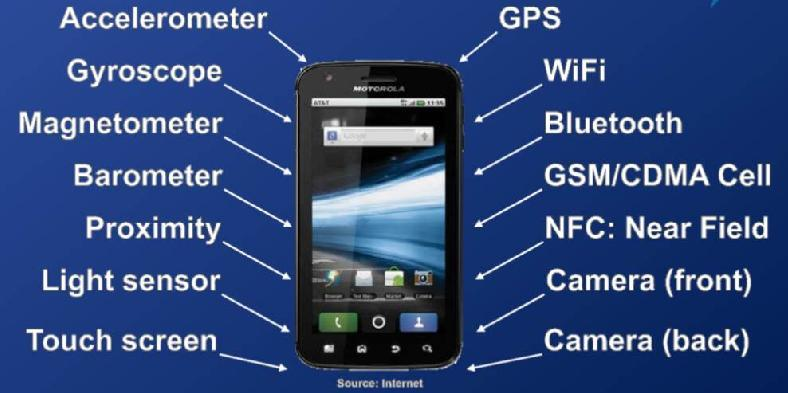
\includegraphics[keepaspectratio, scale=1]{Imagenes/Imagen1.jpg}
\caption{Sensores de un Smartphone.}
\end{figure}


%%\item {Conmutatividad: }La convolucion es conmutativa.
Hoy en día, con las diferentes funciones de los teléfonos inteligentes, algunas como: rastrear, medir el pulso cardiaco, entre otros. Se utilizan diferentes sensores.

\enskip 

Enlistados los sensores más comunes que se encuentran en un smartphone son:
Acelerómetro, giroscopio, magnetómetro, GPS, sensor de proximidad, sensor de luz ambiental, micrófono, sensor de pantalla táctil, sensor de huella digital, podómetro, sensores de código de barras y QR, barómetro, sensor de frecuencia cardiaca, termómetro, sensor de humedad del aire, etc.


\section{Localización en entornos interiores:}

\begin{itemize}
%%\item {Conmutatividad: }La convolucion es conmutativa.
\item Los sistemas de localización en para espacios interiores han tomado importancia conforme a la
introducción de nuevas tecnologías. Estos sistemas introducen mejoras en la seguridad en centros
residenciales, así como en hospitales, centros empresariales, etc.

\end{itemize}


\subsection{Tecnologías para la localización de interiores:}    

\begin{itemize}

%%\item {Conmutatividad: }La convolucion es conmutativa.
\item {WI-FI: }Es una tecnología que permite el traspaso de datos de manera inalámbrica. El WI-FI al se basa
en ondas de radio, de la misma manera que la radio convencional, no obstante, las frecuencias que
manejan son diferentes. La frecuencia utilizada para WI-FI ronda los 5 GHz.

\enskip

\item {BLE: }El bluetooth Low Energy, es un derivado de Bluetooth v4.0 este se utiliza en aplicaciones de
baja potencia. Su mayor ventaja está en la compatibilidad que este tiene en plataformas como IOs,
Android, Microsoft y Linux, otra de sus ventajas el tamaño reducido que suelen tener estos
dispositivos, de esta manera, facilitado su instalación.


\enskip 

\item {IMU: }Unidad de medida inercial. Es un dispositivo que obtiene información del movimiento,
orientación, fuerzas gravitacionales. La información que obtenemos de ellos se ve representada por
tres valores numéricos que están relacionadas con los siguientes tres dispositivos: Acelerómetro,
Giroscopio y Magnetómetro.

\enskip

Las componentes de IMU, dependiendo de cuantos dispositivos tengan pueden constar de tres a nueve
ejes. Siendo tres si solo cuentan con uno de los dispositivos, acelerómetro, giroscopio, magnetómetro;
seis si cuentan con dos de ellos y nueve, si cuentan con los tres.

\enskip

\item {RSSI: }Es una medida aproximada de lo que un dispositivo puede detectar. Lo bueno de RSSI es que
le ayuda a determinar y saber si una señal es suficiente para establecer una conexión inalámbrica. Este
RSSI suele ser invisible para el usuario de un dispositivo receptor, pero como la intensidad de la señal
varia enormemente y afecta a la función de una conexión inalámbrica, los dispositivos a veces ponen
la medida a disposición de los usuarios.

\end{itemize}

 \section{Beacon Bluetooth:}

 %%\item {Conmutatividad: }La convolucion es conmutativa.
 Un Beacon, en español baliza, es un dispositivo transmisor de radio, de un tamaño reducido. Estos
pequeños dispositivos mandan si parar señales BLE (Bluetooth de baja energía). Tecnología Bluetooth
con la que cuentan los smartphones.

\enskip

Tecnología relevante para la transferencia de información, transmitir anuncios en centros comerciales,
parques de atracciones, entre otros.
 

 
 \subsection{Beacon Bluetooth del fabricante Estimoté:}
 

 Son dispositivos que emiten señales que son recibidas e interpretadas por smartphones, dispositivo
alimentado por una batería, consta de un procesador ARM, memoria, sensores de temperatura,
bluetooth y sensores de movimiento.

\enskip

Cada beacon envía un ID único de tal manera que pueda ser identificado por otros dispositivos, cada
ID contiene 20 bytes y nuestros smartphones pueden detectar múltiples beacons a sus alrededores y
clasificarlos ya sea por ID o por distancia.

\enskip

Se utilizan normalmente en centros comerciales, ubicados en la parte de afuera de los negocios,
anunciando descuentos, ofertas, etc.

\enskip

Los componentes necesarios para que un teléfono móvil pueda recibir señales de este dispositivo
beacon bluetooth son:

\begin{itemize}
    \item BLE.
    \item WI-FI.
    \item IOs 7, Andorid 4,3 o superior.
    \item Aplicativo Móvil.
\end{itemize}



%%\clearpage
Ficha técnica:

\begin{itemize}
    \item Beacon de proximidad.
    \item Beacon de Localización.
\end{itemize}

\clearpage

\begin{figure}[H]
\centering
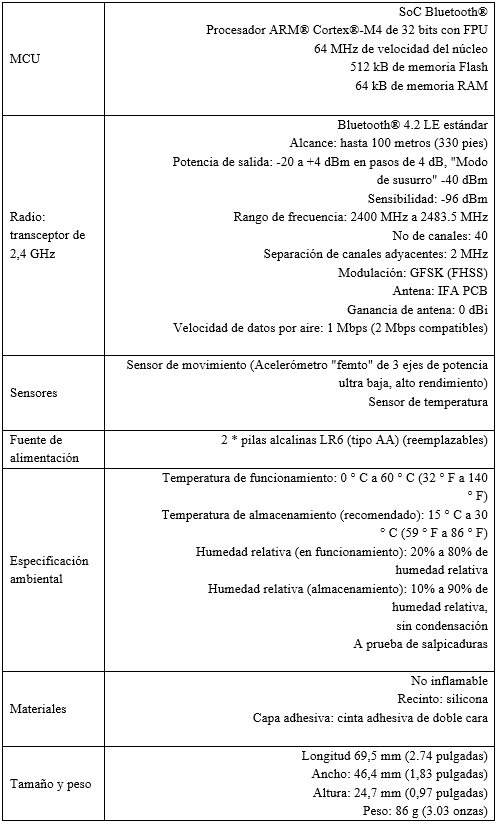
\includegraphics[keepaspectratio, scale=1]{Imagenes/Imagen2.png}
\caption{Ficha técnica beacon de proximidad.}
\end{figure}

\clearpage

\begin{figure}[H]
\centering
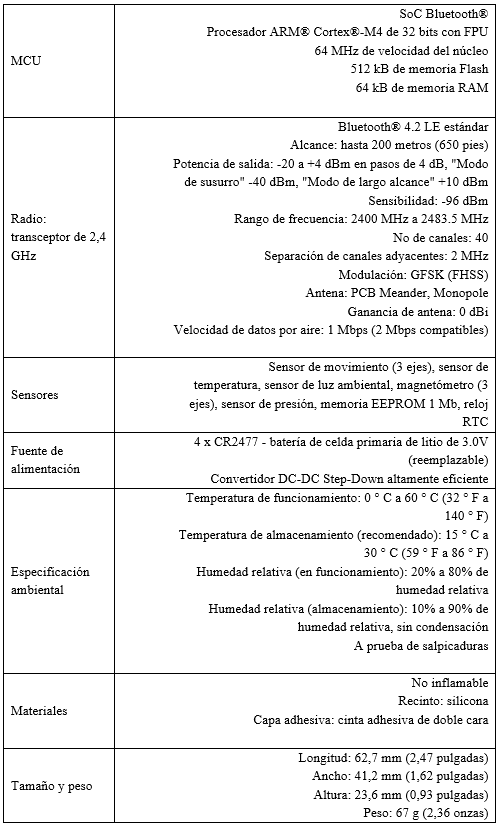
\includegraphics[keepaspectratio, scale=1]{Imagenes/Imagen3.png}
\caption{Ficha técnica beacon de localización.}
\end{figure}


 

\subsection{Trama de una señal BLE, protocolos iBeacon y Eddystone:}        
         
 \begin{itemize}
 \item{iBeacon: }Es un protocolo inalámbrico de Apple en base a BLE (Bluetooth de baja intensidad). Permite una señal bluetooth de hasta 30 metros entre smartphones, utilizado en las tiendas estadounidenses para realizar pagos entre clientes y tiendas.
 
 \enskip
 
 La tecnología detrás de iBeacon se basa en el modelo simple de transmisor y receptor, o tecnología Beacon. 
 
  \enskip
  
  En un espacio determinado se instalan transmisores, los llamados beacons. Una vez que un receptor es detectado por una baliza, el transmisor mide la intensidad de la señal del dispositivo y determina su UUID, un código utilizado para identificar dispositivos en una red. 
  
  \enskip
  
  Comparado con la tecnología de transmisión inalámbrica, el iBeacon se basa en la tecnología Bluetooth Low Energy. Los iBeacons presentan una alternativa de menor coste a la tecnología NFC. Apple introdujo por primera vez el protocolo iBeacon en 2013 en algunas de sus tiendas de Estados Unidos.
  
  \enskip
  
  iBeacon puede ser usado por dispositivos iOS7 y Android 4.3 en adelante. Estos dispositivos con compatibles con el estándar inalámbrico.
  
  \enskip
 
 \item{Eddystone: }En 2015 Google lanzó este protocolo, tiene compatibilidad tanto con teléfonos iOS como con teléfonos Android.
 
 \enskip
 
 Todas las normas de uso de su propia estructura de la publicidad BLE para añadir sus datos y formatos. Por lo tanto, todo el explorador de paquetes BLE o receptor puede recoger ese paquete fácil. Una vez que el receptor recibe, se determina que, o bien que el paquete es descifrable o no.
 
 \enskip
 
 Dentro de la trama se definen, longitud, tipo, y datos. La longitud define le tamaño de los campo de datos, el tipo de dato define la estructura de este y su uso posterior, y los datos hacen referencia a la cadena que se va a transmitir.

 \end{itemize}
 
 \begin{figure}[H]
\centering
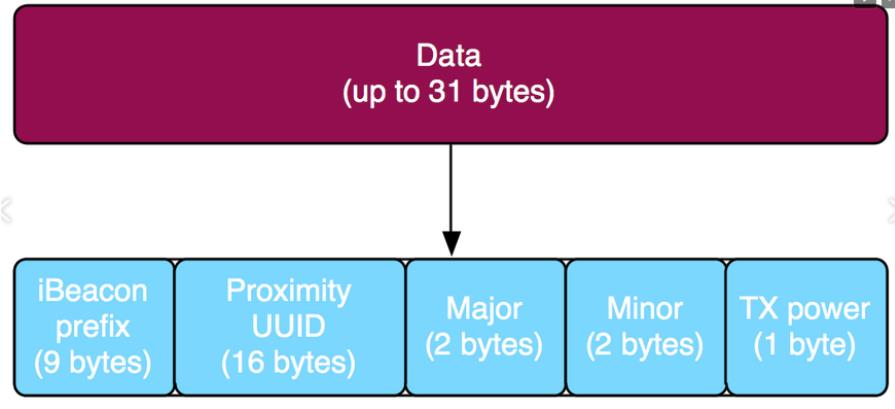
\includegraphics[keepaspectratio, scale=1]{Imagenes/Imagen4.jpg}
\caption{Trama BLE protocolos iBeacon, Eddystone}
\end{figure}

\section{Trama de red WI-FI:}
Viene a ser el equivalente de paquete de datos o Paquete de red, en el Nivel de red del modelo OSI.

\section{Desarrollo móvil.}

\subsection{Desarrollo nativo:}


    El desarrollo de aplicaciones ha sido en los últimos años una de las áreas de la industria con mayores oportunidades.\newline


Existen muchas maneras de desarrollarlas, con lenguajes diversos y plataformas o frameworks creados por distintas compañías, sin embargo, el medio más apropiado para realizar un desarrollo continúa siendo el nativo.\newline


Desarrollo nativo es aquel en el que usamos los lenguajes y tecnologías que ofrece el propio sistema operativo para el que se está programando.\newline


En iOS, el desarrollo nativo se realiza mediante los lenguajes Swift y Objective -C y en Android el desarrollo nativo se realiza usando Java como lenguaje.\newline

El desarrollo nativo es más aconsejable debido a diversos factores:\\

\begin{itemize}
    \item Rendimiento. Pues los lenguajes nativos son mejores aprovechando mejor lo que ofrece el sistema operativo.
    \item Permite usar directamente todos los periféricos disponibles en el dispositivo, como la cámara, acelerómetro, almacenamiento, GPS, linterna, etc., sin la necesidad de plugins o librerías de terceros.
    Y la desventaja de la creación de aplicaciones nativas, es la necesidad de realizar dos proyectos diferentes, lo que duplica el trabajo y exige generalmente equipos de desarrollo distintos, pues los conocimientos necesarios para desarrollar en cada plataforma son muy distintos. 
    
\end{itemize}



\subsection{Aplicaciones web para móviles, ventajas:}




 Son muchas las compañías que no van a dejar pasar la oportunidad de unirse a este negocio y se aventuran a crear una aplicación web que dé respuesta a sus necesidades.\newline

Una aplicación web móvil es aquella que esta diseñada para funcionar tanto en un aplicativo construida a partir de lenguajes nativos destinada a un smartphone, así como también se podrá visualizar desde un navegador web en una laptop.\newline

Está destinada a plataformas como Android, iOS, Windows Phone, siendo estas distintas plataformas se deberá desarrollar la adaptación requerida por cada plataforma según el lenguaje con el que el sistema operativo funcione, dicho de otra forma, crear un aplicativo diferente para cada plataforma.\newline

Ventajas:\\

\begin{itemize}
    \item Acceso completo al dispositivo.
    \item Mejor experiencia de usuario.
    \item Visibilidad en tienda de aplicaciones.
    \item Envío de notificaciones a los usuarios.
    \item La actualización de app es constante.
    \item Código de programación reutilizable.
    \item Desarrollo mas sencillo y a menor costo.
\end{itemize}


 
\subsection{Diagrama de casos del sistema:}


El diagrama de casos del sistema representa como actores, entidades se relacionan dentro de un sistema, asignando diferentes actividades o casos de uso. Dentro del diagrama encontramos: 

\begin{itemize}
    \item Actor.
    \item Casos de Uso.
    \item Relaciones de Uso, herencia y comunicación.
\end{itemize}

\subsection{Diagrama de actividades:}
Muestra las actividades que deben ser realizadas en un caso de uso, como también las relaciones de uso y como deben estar direccionadas.\newline

Es importante recalcar que aunque un diagrama de actividad es muy similar en definición a un diagrama de flujo, no son lo mismo. Un diagrama de actividad es utilizado en conjunción de un diagrama casos de sistema para auxiliar a los miembros del equipo de desarrollo a entender como es utilizado el sistema y cómo reacciona en determinados eventos. Se pudiera considerar que un diagrama de actividad describe el problema, mientras un diagrama de flujo describe la solución\newline

En el diagrama de actividades encontramos:

\begin{itemize}
    \item Inicio.
    \item Actividad.
    \item Transición.
    \item Ramificación.
    \item Unión.
    \item Expresiones Resguardadas.     
    \item Fork.
\end{itemize}

\subsection{Requerimientos de Software:}

Su gestión efectiva contribuye a mejorar la calidad y reutilizar esfuerzos en las distintas actividades de un proyecto de software.\newline

Actualmente, existen diversas técnicas para mejorar la calidad y efectividad de las actividades de desarrollo, mantenimiento, pruebas, etc.\newline

Sin embargo, considerando el papel central de los requisitos, es importante definir e implantar una estrategia de obtención, especificación, validación y gestión de requisitos.\newline

Todo ello tiene como misión favorecer la calidad de estas actividades en base a un repositorio común del conocimiento del sistema, que tenga como eje una estrategia adecuada y transversal de ingeniería de requisitos.

\section{Google App Engine:}

Google App Engine, ofrece un servicio de alojamiento web gratuitito en primera instancia, esta opción ofrece hasta 500 Mb de almacenamiento, el cual se puede mejorar con tarifas mensuales.\newline 

En App Engine podemos utilizar un dominio propio, o bien el que ofrece con la estructura: nombre.appspot.com. Google App Engine ofrece lo siguiente:

\begin{itemize}
    \item Un servidor web dinámico, compatible con las tecnologías web más habituales.
    \item Distribución de cargas y escalado automático.
    \item Almacenamiento permanente
    \item Entorno de desarrollo local para simular en nuestro equipo Google App Engine.
    \item API para enviar correo y autenticar usuarios mediante Google Accounts.
    \item Tareas programadas y colas de tareas.
    \item Los lenguajes de programación que utiliza Google App Engine son Java y Python.
\end{itemize}

Entre las ventajas que tiene App Engine, se encuentran: Desarrollar la aplicación es gratuito y muy sencillo, está a la disposición de todo el mundo, se puede buscar un presupuesto que se acomode a las necesidades del desarrollador, se puede desarrollar un total de hasta diez aplicaciones, y sus recursos apreciados por muchos desarrolladores son muy útiles.

\section{Bases de datos:}

Se denomina base de datos, a un conjunto de información perteneciente a un mismo contexto, ordenada de modo sistemático para su posterior recuperación, análisis y/o transmisión.\newline 

Existen actualmente diversas formas de bases de datos, que van desde una biblioteca hasta los vastos conjuntos de datos de usuarios de una empresa de telecomunicaciones.

Las bases de datos son el producto de la necesidad humana de almacenar la información, es decir, de preservarla contra el tiempo y el deterioro, para poder acudir a ella posteriormente.\newline  

El manejo de las bases de datos se lleva mediante sistemas de gestión, actualmente digitales y automatizados, que permiten el almacenamiento ordenado y la rápida recuperación de la información. En esta tecnología se halla al principio de la informática.\newline 

En la conformación de una base de datos se pueden seguir diferentes modelos y paradigmas, cada uno dotado de características, ventajas y dificultades, haciendo énfasis en su estructura organizacional, su jerarquía, su capacidad de transmisión o de interrelación, etc.\newline 

Esto se conoce como modelos de base de datos y permite el diseño y la implementación de algoritmos y otros mecanismos lógicos de gestión, según sea el caso específico.\newline 

\subsection{SQL:}

Las bases de datos relacionales con una recopilación de distintos elementos, entidades y actores que relacionan entre sí. Estos elementos se organizan en tablas con filas y columnas. \newlineew

Cada columna de una tabla guarda un determinado tipo de datos y un campo almacena el valor real de un atributo. Cada fila de una tabla podría marcarse con un identificador único denominado clave principal, mientras que filas de varias tablas pueden relacionarse con claves extranjeras.\newline

\subsection{SQL Lite:}

Es una biblioteca desarrollada en lengua C que implementa un SGBT (sistema gestor de bases de datos transaccionales). Carecen de servidor y configuración.\newline

SQL Lite es público y libre para el uso que se deseé, uso comercial o privado. Utilizado actualmente por gran cantidad de aplicaciones de alto nivel.  \newline

\section{8.	Avance y segunda entrega:}

\subsection{Pantallazo Aplicación Android Stusedio Main Activity:}

 \begin{figure}[H]
\centering
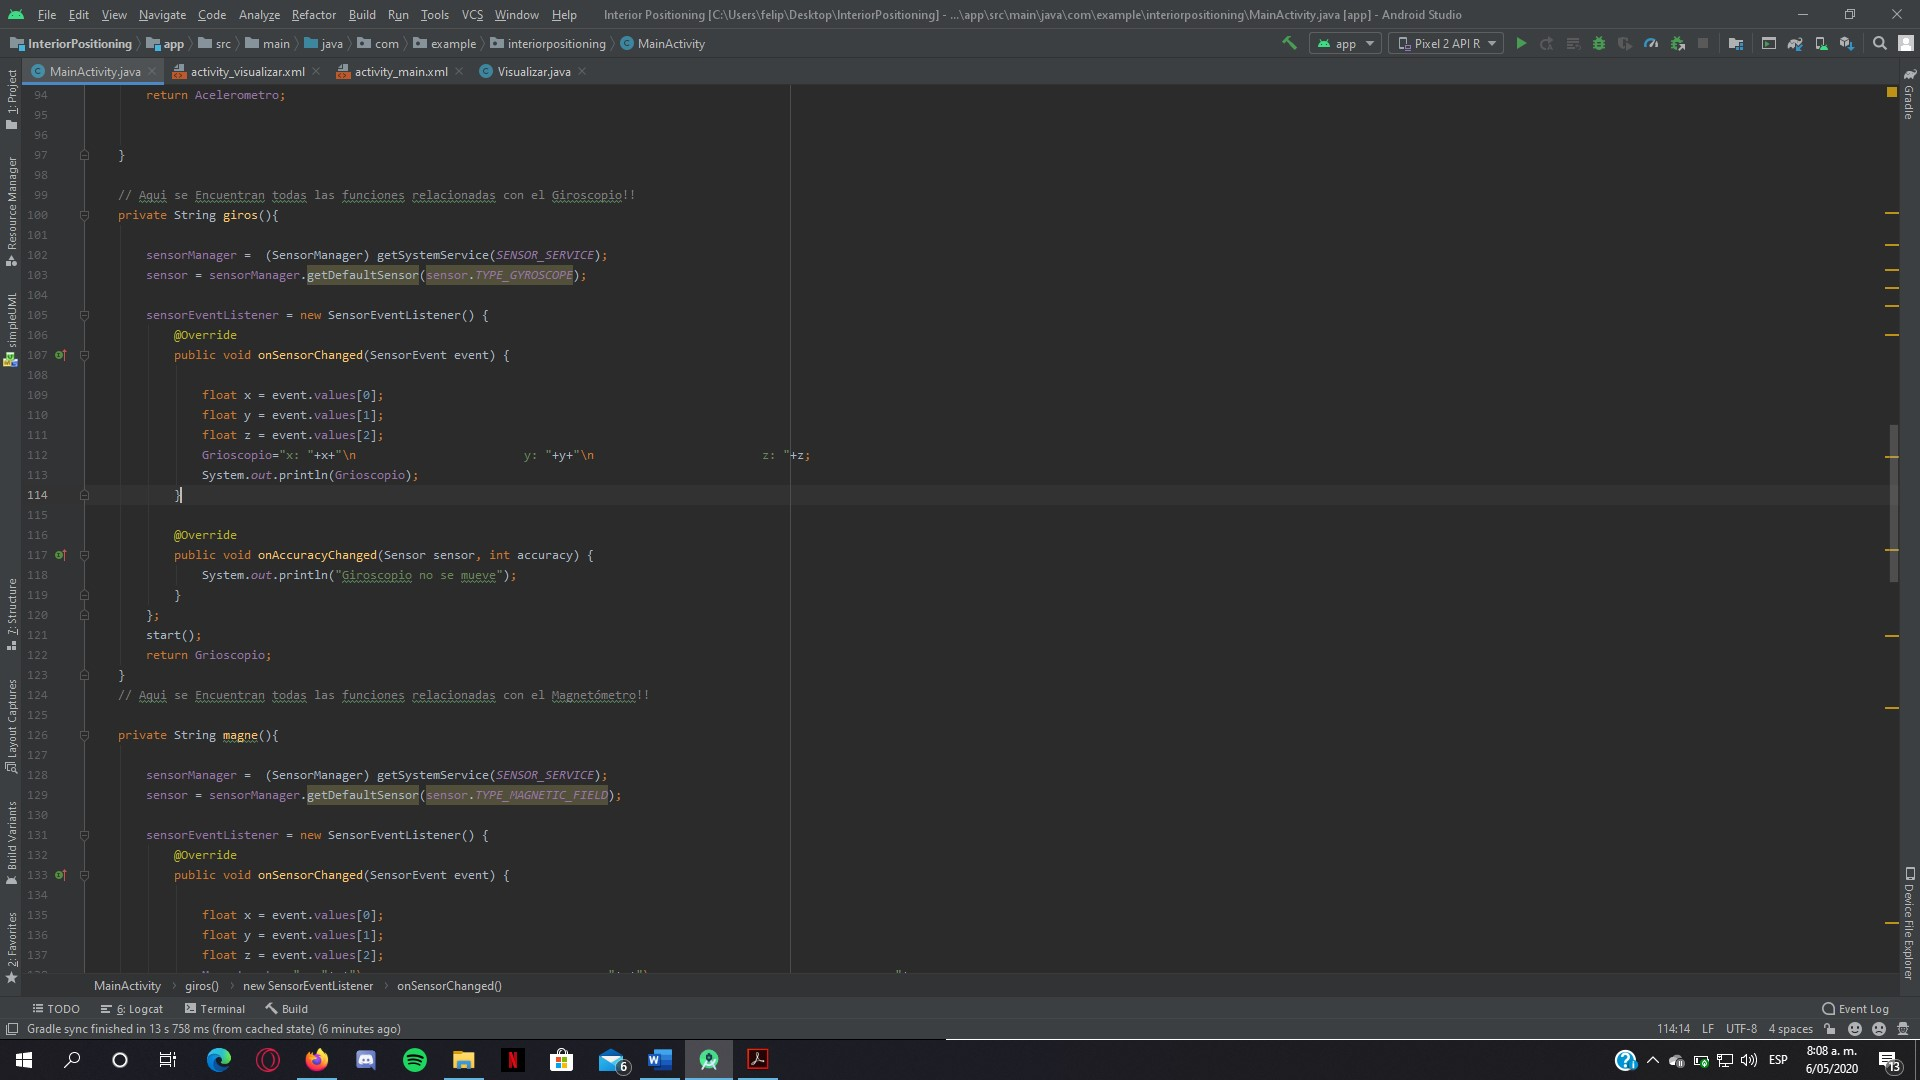
\includegraphics[keepaspectratio, scale=0.5, width=\textwidth]{Imagenes/Imagen5.jpg}
\caption{Pantallazo clase principal Android Studio}
\end{figure}

\subsection{Pantallazo Aplicación Android Studio Base de datos:}

 \begin{figure}[H]
\centering
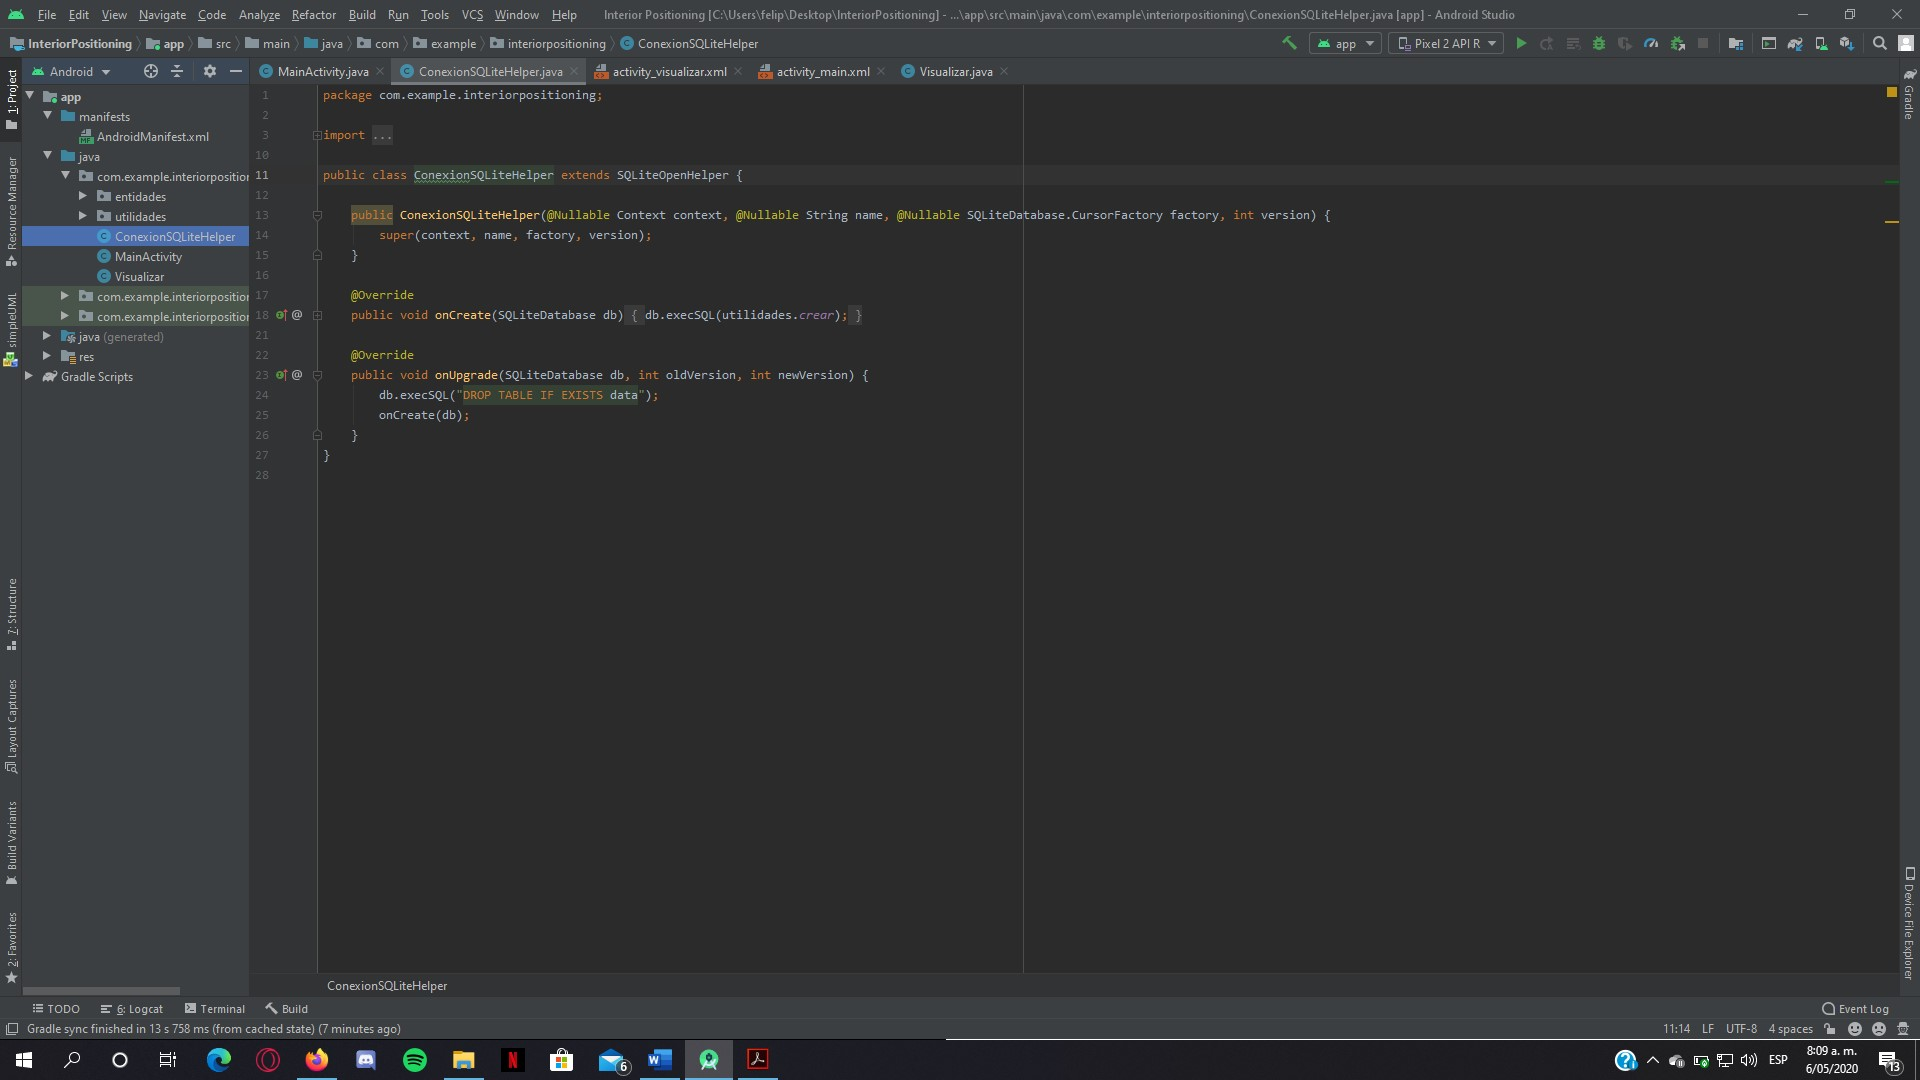
\includegraphics[keepaspectratio, scale=0.5, width=\textwidth]{Imagenes/Imagen6.jpg}
\caption{Pantallazo clase conexión base de datos:}
\end{figure}
\enskip
\subsection{Modelo de casos de uso:}

 \begin{figure}[H]
\centering
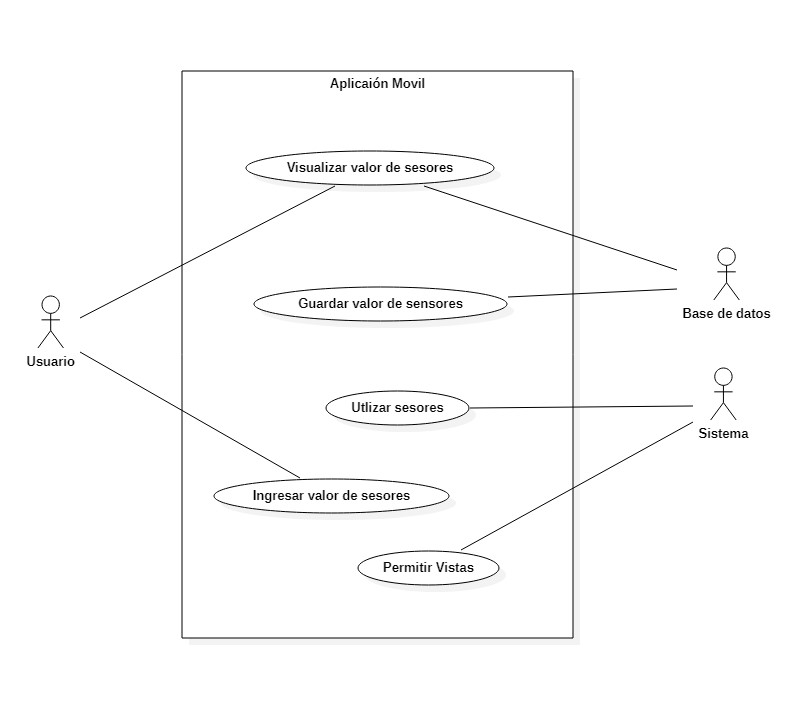
\includegraphics[keepaspectratio, width=400pt ,height=239pt]{Imagenes/Imagen7.jpg}
\caption{Modelo de casos de uso:}
\end{figure}

\subsection{Modelo de clases:}

 \begin{figure}[H]
\centering
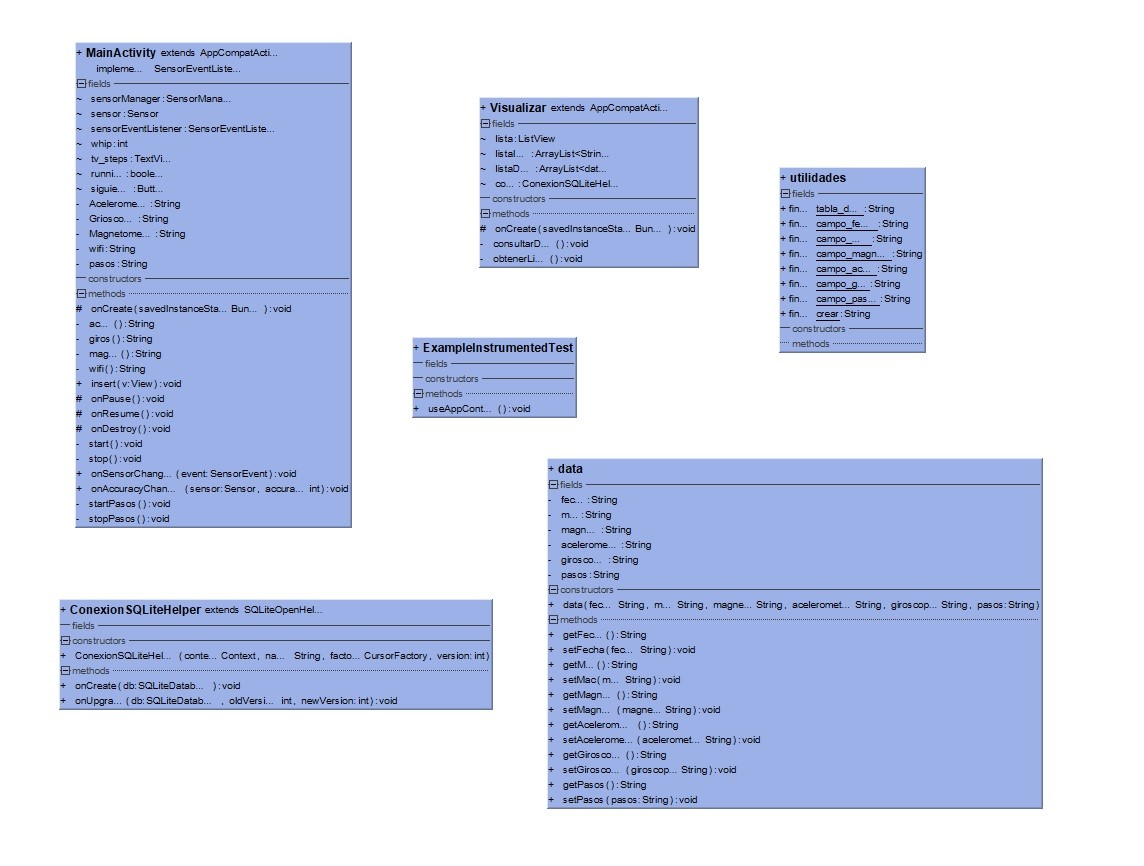
\includegraphics[keepaspectratio, width=\textwidth, height= 338pt]{Imagenes/Imagen8.jpg}
\caption{Modelo de clases de la aplicación}
\end{figure}

\enskip

\subsection{Modelo de Actividades:}

 \begin{figure}[H]
\centering
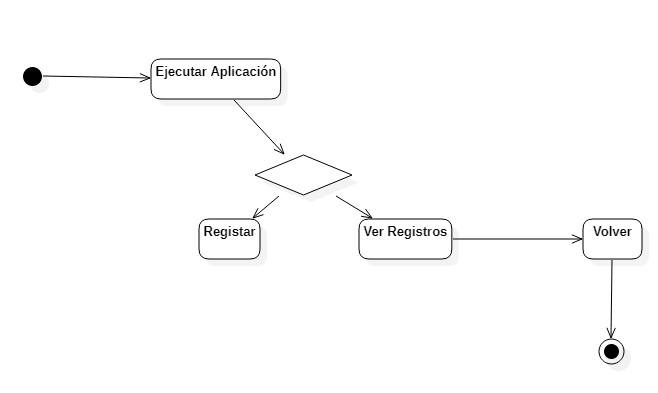
\includegraphics[keepaspectratio, width=400pt ,height=190pt]{Imagenes/Imagen9.jpg}
\caption{Modelo de clases de la aplicación}
\end{figure}

\section{Imágenes, aplicación final:}

\subsection{Vista principal de la aplicación:}
\begin{figure}[H]
\centering
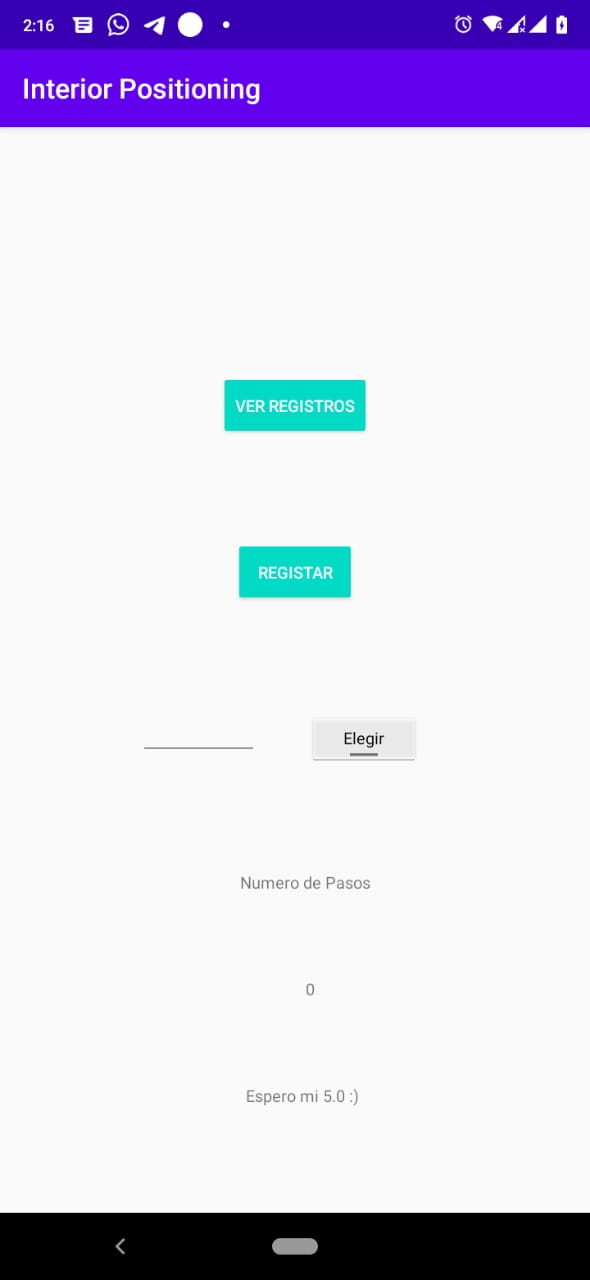
\includegraphics[keepaspectratio, width=400pt ,height=250pt]{Imagenes/imagen10.jpeg}
\caption{Vista principal de la aplicaión (mainActivity)}
\end{figure}
\enskip
\subsection{Vista de las tablas o vista de mostrar registros:}
\begin{figure}[H]
\centering
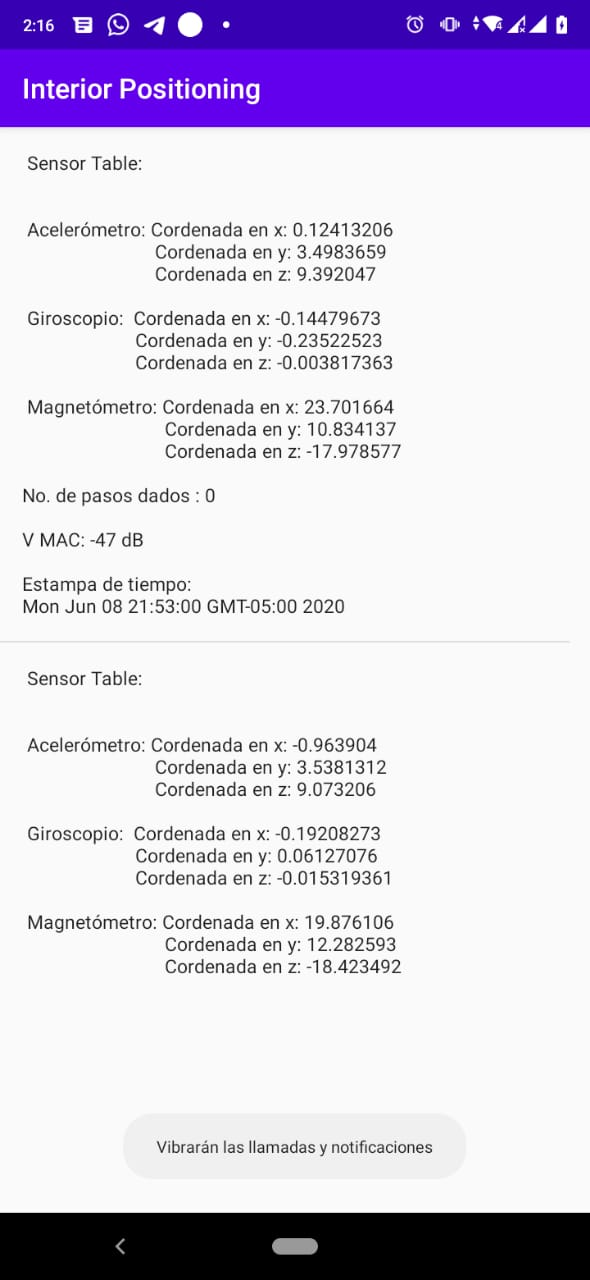
\includegraphics[keepaspectratio, width=400pt ,height=250pt]{Imagenes/imagen11.jpeg}
\caption{VVista de las tablas o vista de mostrar registros (mainVisualizar}
\end{figure}
\enskip
\subsection{Vista botón elegir:}
\begin{figure}[H]
\centering
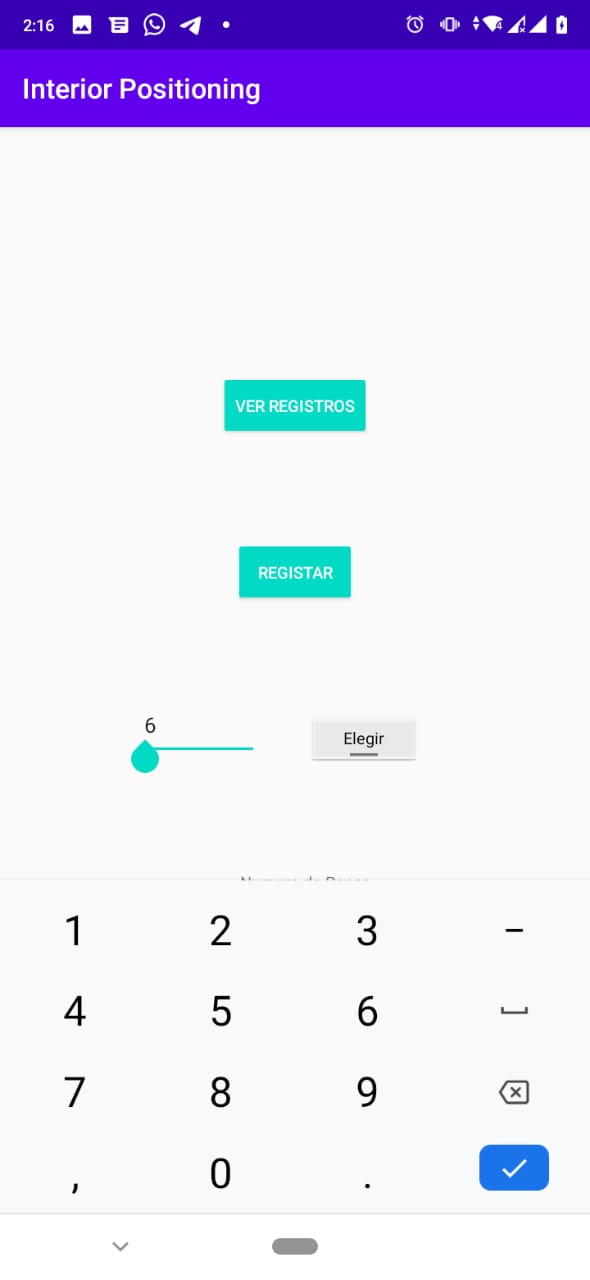
\includegraphics[keepaspectratio, width=400pt ,height=250pt]{Imagenes/imagen12.jpeg}
\caption{Vista botón elegir (buttonElegir)}
\end{figure}
\enskip
\subsection{Vista botón elegir bloqueada:}
\begin{figure}[H]
\centering
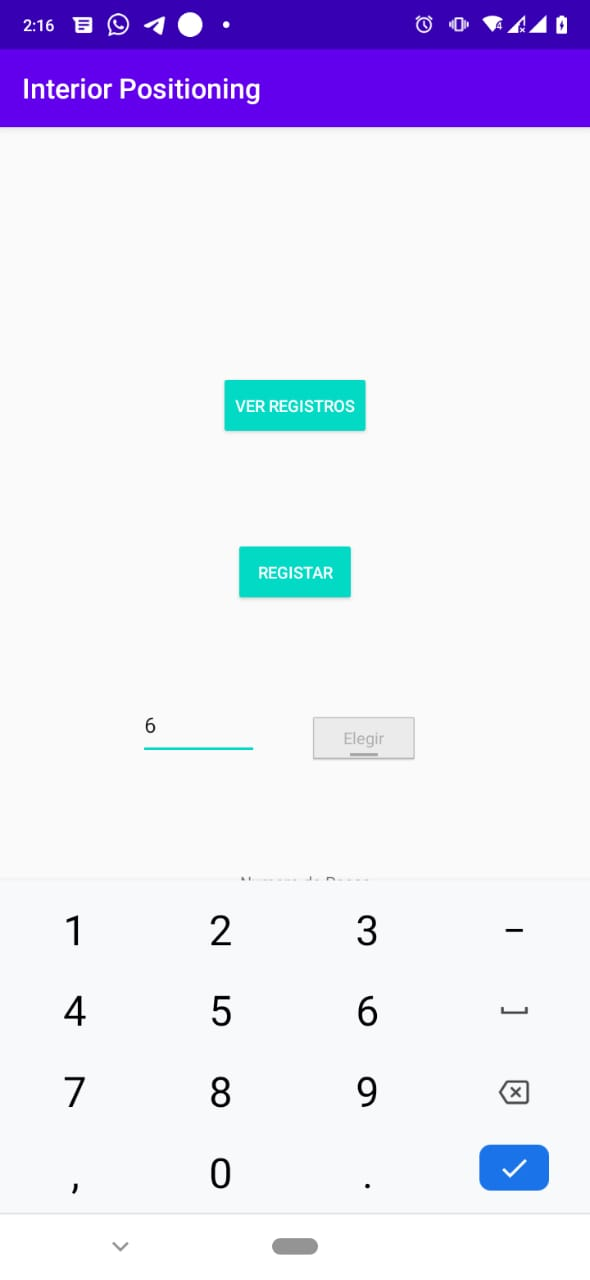
\includegraphics[keepaspectratio, width=400pt ,height=250pt]{Imagenes/imagen13.jpeg}
\caption{Vista botón elegir bloqueada (buttonElegir, enable = false)}
\end{figure}


\section{Conclusión}

Gracias a los conceptos que se encuentran en la anterior investigación, tenemos certeza de que tipo de sensores se encuentran en un teléfono inteligente / smartphone, estos mejoran la experiencia del usuario con su dispositivo. De igual forma se identificaron las tecnologías usadas para la localización en entornos digitales, BLE, WI-FI, RSI, entre algunos otros, su uso en diferentes entornos y su implementación móvil.\newline

Se entiende como el funcionamiento del bluetooth de baja energía, así como también los del dispositivo Beacon de los fabricantes Estimoté y la composición de la trama que utilizan tanto iBeacon, como Eddystone.\newline

Para el desarrollo de una aplicación se debe conocer el entorno y la problemática que va a solucionar el producto a desarrollar. Para este fin, herramientas como los diagramas de actividades, casos de uso y los requerimientos del software.\newline

Se ha concluido que aplicaciones hibridas que funcionen en diferentes plataformas es la mejor opción para que el usuario la pueda usar sin importar el tipo de dispositivo con el que cuente; iOS, Android o Windows Phone. Ahí la importancia del desarrollo nativo de las aplicaciones pues son lenguajes básicos, fáciles de utilizar y compatibles en las plataformas más usadas. También nos encontramos con opciones como App Engine de Google que facilita el desarrollo de aplicaciones gratuitas y que alcancen a todo público.\newline

Finalmente se entiende el concepto de base de datos y los diferentes tipos que existen, así como las opciones libres como SQL Lite que se encuentran para un desarrollo sin barreras económicas que pueda tener una aplicación.\newline

La aplicación Andorid Studio, es por excelencia la mejor si el objetivo es desarrollar aplicaciones destinadas a dispositivos con sistema operativo Android. Sin embargo, se tuvieron infinidad de problemas pues esta aplicación pide demasiados recursos a la computadora, sin mencionar que para el ejercicio no se utilizo la virtualización que ofrece el IDE. Se utilizo un celular en modo depuración conectado con el Software Andorid Studio.

Utilizar una herramienta en este caso una API de Google como Firebase para el uso de base de datos y almacenamiento en la nube resulta acertado y mas aún cuando trabajamos con aplicaciones Android. Firebase es perfectamente compatible con Android gracias que ambas tanto Android, como Firebase son de la misma empresa, Google.\newline

La gestión de los datos resulta más manejable para un futuro gestor de bases de datos, la plataforma es simple de usar e inclusive mucho más fácil de gestionar gracias a la API de Google.\newline

Por último, es importante decir que plataformas como Asure de Microsoft, Firebase de Google, Amazon web service, entre otras, son excelentes para nuevos como desarrolladores y/o arquitectos ya experimentados en lo que a pruebas de aplicación se refiere.\newline

\section{Respositorio, GitHub y Video}
\href{https://github.com/FelipeUribe81/SignalAnalysis}{} A continuación se encuentra el link del repositorio en GitHub: \url{https://github.com/FelipeUribe81/SignalAnalysis}\newline

\href{https://www.youtube.com/watch?v=p6pmw7bPFvY}{} A continuación se encuentra el link del vidoe en Youtube: \url{https://www.youtube.com/watch?v=p6pmw7bPFvY}\newline


\begin{thebibliography}{0}
  \bibitem{Cuwhois} Cuwhoi, 26 10 2018. [En línea]. Available: http://www.cuwhois.com/tecnologia/cuantos-sensores-tiene-tu-smartphone.php.\newline
  
  \bibitem{NGD (Negocios y Gestión de dependencia)} NGD (Negocios y Gestión de ,dependencia). 21 05 2019. [En línea]. Available: https://gestionydependencia.com/noticia/2542/actualidad/asi-funciona-el-sistema-de-localizacion-en-interiores-de-ibernex.html. \newline
                             
   \bibitem{ELT, innovation in lighting tecnology}ELT, innovation in lighting tecnology. SF. [En línea]. Available: https://www.elt.es/ble-bluetooth-low-energy.\newline
   
   \bibitem{Beaconstac}Beaconstac, 2020. [En línea]. Available: https://www.beaconstac.com/what-is-a-bluetooth-beacon.\newline
   
   \bibitem{Estimote}Estimote, 2018. [En línea]. Available: https://community.estimote.com/hc/en-us/articles/204092986-Technical-specification-of-Estimote-Beacons-and-Stickers.\newline
   
    \bibitem{Blascarr}Blascarr, 2020. [En línea]. Available: http://blascarr.com/lessons/introduccion-al-imu-sistemas-de-navegacion-inercial.\newline

    \bibitem{Escuela IT}Escuela IT, S.F. [En línea]. Available: https://escuela.it/materias/desarrollo-nativo.\newline
    
    \bibitem{RyteWiki}RyteWiki, S.F. [En línea]. Available: https://es.ryte.com/wiki/iBeacon.\newline
    
    \bibitem{MOKOSMART}MO,KOSMART,ioT Designer y Manufacturer, 10 2019. [En línea]. Available: https://www.mokosmart.com/es/eddystone-protocol-and-specifications.\newline

    \bibitem{LanceTalent}LanceTalent, 20 02 2014. [En línea]. Available: https://www.lancetalent.com/blog/tipos-de-aplicaciones-moviles-ventajas-inconvenientes.\newline
    
    \bibitem{Omosis Latina.}Omsis Latina, S.F. [En línea]. Available: https://www.osmosislatina.com/lenguajes/uml/actividad.htm.\newline
    
    \bibitem{ N. A. y. a. D. UNAD}. N. A. y. a. D. UNAD, Stadium Unad, S.F. [En línea]. Available: http://stadium.unad.edu.co/ovas/105969839/diagramasdecasosdeuso.html.\newline

    \bibitem{Sogeti}Sogeti, S.F. [En línea]. Available: https://www.sogeti.es/soluciones/calidad-de-software/servicios-de-testing/formacion-testing/curso-requisitos-de-software.\newline

    \bibitem{DIGIWORKS}F. Brugman, DIGIWORKS, S.F. [En línea]. Available: https://www.digiworks.es/que-es-google-app-engine-y-para-que-sirve/.\newline
    
    \bibitem{Amazon}Amazon, S.F. [En línea]. Available: https://aws.amazon.com/es/relational-database/.\newline
    
    \bibitem{Amazon}Amazon,  S.F. [En línea]. Available: https://aws.amazon.com/es/relational-database/.\newline
    
    \bibitem{EcuRed}EcuRed, S.F. [En línea]. Available: https://www.ecured.cu/SQLite.\newline
    
    \bibitem{Speedcheck}Speedcheck, S.F. [En línea]. Available: https://www.speedcheck.org/es/wiki/rssi/.

\enskip

\end{thebibliography}


\end{document}


